\documentclass[english, 12pt]{scrartcl}
\usepackage[utf8]{inputenc}
\usepackage{amsmath}
\usepackage{amsthm}
\usepackage{amssymb}
\usepackage{dsfont}
\usepackage{enumitem}
\usepackage{tikz}
\usepackage{pgfplots}
\usepackage[onehalfspacing]{setspace}
\usepackage{float}

\theoremstyle{definition}
\newtheorem{example}{Example}[section]

\theoremstyle{definition}
\newtheorem{definition}{Definition}

\theoremstyle{definition}
\newtheorem{theorem}{Theorem}

\begin{document}

% TODO title, "Total preorder in the courtroom"?
\title{Of judges, aliens and tpos}
\subtitle{Report on 'How to Revise a Total Preorder' \cite{Booth2011} for seminar 1901 - 'Representation and processing of uncertain knowledge with logic-based methods'}
\author{
	Heltweg, Philip (3230880) \\
	University of Hagen \\
	pheltweg@gmail.com
}
\date{\today}
\maketitle

\abstract{Total preorders are a common tool to model plausibility orderings over worlds for agents in the research field of belief change. In their paper 'How to Revise a Total Preorder', Booth and Meyer present an approach to revising preorders for iterated belief revision based on assigning abstract intervals of plausibility under new evidence to worlds.

This report presents part of their work in tpo-revision operators and their properties with the help of an accompanying example and additional visualisation.}

\newpage

\tableofcontents

\newpage

\section{Introduction}

In the field of belief change total preorders (or tpos) are a common tool to model an agent's conditional beliefs. To support iterated belief revision it is necessary to research how these structures can be changed to adapt to an agent's changing world view.
Booth and Meyer suggest an approach based on the idea of assigning an interval of additional metadata to the ordered, propositional worlds and iterate the tpo of an agent using that structure. They define and discuss properties of operators for tpo-revision and relate their approach to other fields of research.
This report on their paper aims to present parts of their work to a wider audience with the addition of an accompanying example. The report's focus will be on the tpo-revision operators discussed in the paper and explicitly avoid the addition of strict preference hierarchies and relations to other research areas.
The structure of the report will be as follows: First it will establish the context of the paper by presenting the research area of iterated belief revision and how it relates to other areas of artificial intelligence and philosophy. To establish a shared understanding of notation and definitions section \ref{section:formal-background} will discuss formal background and other, previous approaches to belief change. It will also introduce the main contribution of this report in an accompanying example demonstrating tpo-revision as described by Booth and Meyer. After establishing a foundation, section \ref{section:booth-and-meyer-tpo-revision-operators} and \ref{section:properties-of-bm-tpo-revision-operators} present part of the work from the original paper 'How to Revise a Total Preorder' \cite{Booth2011}. Section \ref{section:booth-and-meyer-tpo-revision-operators} establishes and defines functions $\ast$, used to revise tpos, a core contribution of Booth and Meyer. In section \ref{section:properties-of-bm-tpo-revision-operators} properties of these functions will be presented. To provide an outlook for the additional work done by Booth and Meyer, \ref{section:iterating-preceq-revision} shows their suggestion for a concrete operator for tpo-revision and includes several examples and novel visualisations of it being applied in the context of the accompanying example. Finally section \ref{section:discussion} closes the report with a summary and commentary on Booth and Meyer's approach to iterated belief revision with interval orderings.

\subsection{Research context}
A core process for an agent dealing with uncertain knowledge is updating their worldview when new information becomes available, also called belief change. As an agent can be human or a machine, work in belief change has impact on both philosophy and artificial intelligence \cite{Ferme2011}. Different approaches to handling belief change have been discussed with notable approaches including nonmonotonic logic, probabilistic reasoning and belief revision \cite{Darwiche1997}.

In belief revision, belief change is modelled using an operator that produces an updated set of beliefs from the state of an agent and new evidence. Research in this area discusses appropriate formalisations of agent state and constrains on individual operators or families of operators. Depending on if the suggested operator handles only one new evidence or multiple new evidences the approaches are called one-step or iterated belief revision.

%Consider a knowledge base (KB) represented by a set of sentences in a
%language L. As our perception of the world described by the knowledge base
%changes, the knowledge base must be modified. G~irdenfors [9] distinguishes
%several kinds of modifications. If we simply acquire additional knowledge
%about the world, and the new knowledge does not conflict with the current
%beliefs t of the KB, we expand the KB. If, however, the new knowledge is
%inconsistent with the old beliefs, and we want the KB to be always consistent,
%we must resolve the conflict somehow; this operation will be called revision. A
%* Part of this work was performed while this author was visiting the University of Toronto.
%** This author is partially supported by the Natural Science and Engineering Research Council
%of Canada.
%1 We use the terms belief and knowledge interchangeably in this paper.
%0004-3702/91/$03.50 © 1991 -- Elsevier Science Publishers B.V. All rights reserved 
%264 H. Katsuno, A.O. Mendelzon
%different kind of change occurs when a sentence previously believed becomes
%questionable and has to be given up; the operation that makes this change is a
%contraction

% TODO: discussed in \cite{Katsuno1991} correct? was mentioned in intro of Admissible and Restrained Revision
A common tool used to encode plausibility assumptions of an agent about possible worlds are total preorders (shortened as tpos) \cite{Booth2011}, discussed in \cite{Katsuno1991}. The primary article for this report, 'How to Revise a Total Preorder', researches how to model the change of these total preorders when new evidence becomes available. Being able to derive a new tpo from additional evidence is an approach to handling multiple revision steps and therefor places the article in the field of iterated belief revision.

\section{Formal background}
\label{section:formal-background}

\subsection{Propositional Logic} % Aussagenlogik
Notation follows as used in \cite{Booth2011}: A propositional language $L$ generated from finitely many propositional variables, lower case greek letters represent formulae in $L$ and $\top$, $\bot$ representing tautology and contradiction respectively. $\vdash$ as classical logical consequence, $\equiv$ classical logical equivalence. $Cn$ is used to denote the deductive closure of a formula or set of formulae in $L$.

$W$ is the set of propositional worlds (also called propositional interpretations in classical logic \cite{Kai2020}). Given a $\alpha \in L$ the set of worlds that satisfy $\alpha$ is denoted by $[\alpha]$.

For any set of worlds $S \subseteq W$ of worlds, $Th(S)$ is the set of sentences true in all worlds in $S$.
% TODO Th(S) not needed?

\subsection{Total preorders}
A total preorder is a binary relation $\leq$ (here over the set of propositional worlds $W$) that is total, reflexive and transitive (i.e. for all $x, y, z \in W$ either $x \leq y$ or $y \leq x$, $x \leq x$ and if $x \leq y$ and $y \leq z$ then $x \leq z$).

The symbol $<$ is used to denote the strict part of $\leq$ while $\sim$ represents the symmetric closure of $\leq$ (i.e. $x \sim y$ iff $x \leq y$ and $y \leq x$).

Tpos are a common tool to handle preference orderings over propositional worlds in literature about belief change \cite{Booth2011}.

A helpful visualisation for tpos is described in \cite{Booth2006}. It uses the fact that tpos can be represented as a linearly ordered set of ranks. Each rank of a tpo $\leq$ is defined as the equivalence classes modulo the symmetric closure of $\leq$: $[[x]]_{\sim} = \{y \mid y \sim x\}$. These equivalence classes are then ordered by the relation $[[x]] \leq [[y]]$ iff $x \leq y$

\begin{example}
    \label{example:example-introduction}
    As an accompanying example consider the following situation from a courtroom, closely aligned to \cite{Booth2011} and \cite{Darwiche1997}: 
    
    Our agent is a judge in a murder trial. John and Mary are suspects. $p$ represents "John is the murderer", $q$ represents "Mary is the murderer" and $r$ represents "the victim is an alien". Possible propositional worlds will be denoted as triplets of 0s and 1s denoting $p$, $q$ and $r$ to be true or false, e.g. the $101$-world stands for John being the murderer and the victim being an alien.
    
    To start the agent believes it is reasonable to assume the murderer acted alone (but is not ruling out both of the accused conspiring). In addition it would be extremely surprising (but not impossible) if the victim was an alien.
    
    
    Consider the propositional worlds $W = \{ 000, 001, 010, 011, 100, 101, 110, 111\}$. A tpo representing the judges assumptions would be $\leq$ with $010 \sim 100 < 000 \sim 110 < 011 \sim 101 < 001 \sim 111$. The equivalent representation as a linearly ordered set of ranks is shown in table \ref{tab:visualising-a-tpo-example}.

    \begin{table}[H]
         \centering
        \begin{tabular}{llll}
        $R_{1}$                      & $R_{2}$                                                                   & $R_{3}$ & $R_{4}$                      \\ \hline
        \multicolumn{1}{|l|}{\begin{tabular}[c]{@{}l@{}}$010$\\ $100$\end{tabular}} & \multicolumn{1}{l|}{\begin{tabular}[c]{@{}l@{}}$000$\\ $110$\end{tabular}} & \multicolumn{1}{l|}{\begin{tabular}[c]{@{}l@{}}$011$\\ $101$\end{tabular}} &
            \multicolumn{1}{l|}{\begin{tabular}[c]{@{}l@{}}$001$\\ $111$\end{tabular}} \\ \hline
        \end{tabular}
        \caption{Visualising a tpo as a linearly ordered set of ranks as done in \cite{Booth2006}}
        \label{tab:visualising-a-tpo-example}
    \end{table}
\end{example}

\subsection{Belief sets and epistemic states}
A belief set is the deductively closed set of propositions an agent accepts as true at any given point in time \cite{Ferme2011}. AGM theory \cite{Alchourron1985} defines postulates for belief sets and their contraction, revision or expansion with new evidence.
% TODO explain contraction, revision, expansion?

%    As our perception of the world described by the knowledge base
%    changes, the knowledge base must be modified. G~irdenfors [9] distinguishes
%    several kinds of modifications. If we simply acquire additional knowledge
%    about the world, and the new knowledge does not conflict with the current
%    beliefs t of the KB, we expand the KB. If, however, the new knowledge is
%    inconsistent with the old beliefs, and we want the KB to be always consistent,
%    we must resolve the conflict somehow; this operation will be called revision. A
%    * Part of this work was performed while this author was visiting the University of Toronto.
%    ** This author is partially supported by the Natural Science and Engineering Research Council
%    of Canada.
%    1 We use the terms belief and knowledge interchangeably in this paper.
%    0004-3702/91/$03.50 © 1991 -- Elsevier Science Publishers B.V. All rights reserved 
%    264 H. Katsuno, A.O. Mendelzon
%    different kind of change occurs when a sentence previously believed becomes
%    questionable and has to be given up; the operation that makes this change is a
%    contraction. Other kinds of operations are discussed in [14].

Darwiche and Pearl \cite{Darwiche1997} argue that working with belief sets is not expressive enough for satisfying results in iterated belief revision. They make the distinction between propositional beliefs (i.e. beliefs the agent accepts and are part of the belief set) and conditional beliefs (i.e. beliefs the agent is prepared to adopt with new evidence).

While the AGM postulates define restrictions on revising propositional beliefs (a core one being the principle of minimal change), they place little restrictions on preserving conditional beliefs. In their paper Darwiche and Pearl use epistemic states, abstract entities that contain all information an agent needs for their reasoning, especially their strategy for belief revision. As conditional beliefs are represented by these strategies, it is necessary to define how to modify the strategy itself when encountering multiple new information \cite{Darwiche1997}.

Belief sets can be extracted from epistemic states (the belief set extracted from an epistemic state $\mathbb{E}$ is denoted as $B(\mathbb{E})$). Darwiche and Pearl show that their version of revision of epistemic states can be modelled with a tpo $\leq_{\mathbb{E}}$, associated with $\mathbb{E}$. Extraction of $B(\mathbb{E})$ is done by considering the lowest ranked worlds (i.e. the most plausible interpretations) under $\leq_{\mathbb{E}}$. The set of propositional sentences that holds in all those worlds is assumed to be the belief set of the agent. For notation let $min(\alpha, \leq_{\mathbb{E}})$ denote the set of minimal models for the propositional formula $\alpha$ under $\leq_{\mathbb{E}}$. Then $[B(\mathbb{E})] = min(\top, \leq_{\mathbb{E}})$ is the set of worlds that are models of the belief set $B(\mathbb{E})$ associated with $\mathbb{E}$.

\begin{example}
    Continuing example \ref{example:example-introduction} it is possible to model an epistemic state $\mathbb{E}$ with the tpo $\leq_{\mathbb{E}}$.
    
    $min(\top, \leq_{\mathbb{E}})$ is the set of worlds on the lowest rank, $\{010, 100\}$. A possible belief set is $B(\mathbb{E}) = \{p \vee q, \neg p \vee \neg q, \neg r\}$ as $[B(\mathbb{E})] = \{010, 100\} = min(\top, \leq_{\mathbb{E}})$. Intuitively this makes sense with the initial assumption that John or Mary are the suspects ($p \vee q$), have acted alone ($\neg p \vee \neg q$) and the victim is not an alien ($\neg r$).
\end{example}

% TODO: do we need to discuss this in ore detail? faithful assignment here:
%Katsuno and Mendelzon [17] propose that an epistemic state Ψ
%should be equipped with an ordering ≤Ψ of the worlds (interpretations), where the compatibility with Bel(Ψ) is ensured by the socalled faithfulness.
%Definition 1 (Faithful Assignment [17]) A function Ψ 
%→≤Ψ that
%maps each epistemic state to a total preorder on interpretations is
%said to be a faithful assignment if and only if:
%(FA1) if ω1 ∈ Ψ and ω2 ∈ Ψ, then ω1 Ψ ω2
%(FA2) if ω1 ∈ Ψ and ω2 ∈  / Ψ, then ω1 <Ψ ω2
%Intuitively, ≤Ψ orders the worlds by plausibility, such that the minimal worlds with respect to ≤Ψ are the most plausible worlds.

\subsection{DP-AGM postulates}
\label{chapter:dp-agm-postulates}
The postulates first introduced by \cite{Alchourron1985} and reformulated for iterated belief revision on epistemic states by \cite{Darwiche1997} are repeated here. $\mathbb{E}$ denotes an epistemic state, $B(\mathbb{E})$ it's associated belief set, $B(\mathbb{E}) + \alpha$ the expansion of $B(\mathbb{E})$ by $\alpha$ and $\ast$ being a belief change operator on epistemic states. 

\begin{enumerate}[wide=0pt, widest=99,leftmargin=\parindent,label = ($\mathbb{E}\!*\!\arabic*$)]
    \item\label{E1} $\qquad B(\mathbb{E}\ast\alpha) = Cn(B(\mathbb{E}\ast\alpha))$
    \item\label{E2} $\qquad \alpha \in B(\mathbb{E}\ast\alpha)$
    \item\label{E3} $\qquad B(\mathbb{E}\ast\alpha)  \subseteq B(\mathbb{E})+\alpha$
    \item\label{E4} $\qquad \textrm{If } \alpha \notin B(\mathbb{E}) \textrm{ then } B(\mathbb{E}) + \alpha \subseteq B(\mathbb{E} \ast \alpha)$
    \item\label{E5} $\qquad \textrm{If } \mathbb{E} = \mathbb{F} \textrm{ and } \alpha \equiv \beta \textrm{ then } B(\mathbb{E} \ast \alpha) = B(\mathbb{F} \ast \beta)$
    \item\label{E6} $\qquad \bot \in B(\mathbb{E} \ast \alpha) \textrm{ iff } \vdash \neg \alpha$
    \item\label{E7} $\qquad B(\mathbb{E} \ast (\alpha \wedge \beta)) \subseteq B(\mathbb{E} \ast \alpha) + \beta$
    \item\label{E8} $\qquad \textrm{If } \neg \beta \notin B(\mathbb{E} \ast \alpha) \textrm{ then } B(\mathbb{E} \ast \alpha) + \beta \subseteq B(\mathbb{E} \ast (\alpha \wedge \beta))$
\end{enumerate}

To guarantee the ability to extract unique belief sets from epistemic states after a revision by $\alpha$, Booth and Meyer \cite{Booth2011} modify these postulates by requiring consistent epistemic inputs. That requirement means dropping \ref{E6} and considering only \ref{E1}-\ref{E5} and \ref{E7}-\ref{E8} as DP-AGM.

While DP-AGM define the most plausible worlds after a revision by $\alpha$ (as $min(\alpha, \leq_{\mathbb{E}})$), Darwiche and Pearl also define postulates that restrict the rest of the new ordering. Because the focus of this report is on the revision of tpos, the semantic (i.e. in terms of how the ordering of worlds undergoes change) versions are shown here, for more details and sentential versions refer to \cite{Darwiche1997}.

\begin{enumerate}[wide=0pt, widest=99,leftmargin=\parindent,label = (CR$\arabic*$)]
    \item\label{CR1} $\qquad \textrm{If } v\in [\alpha], w \in [\alpha] \textrm{ then } v \leq_{\mathbb{E}} w \textrm{ iff } v \leq_{\mathbb{E\ast\alpha}} w$
    \item\label{CR2} $\qquad \textrm{If } v\in [\neg \alpha], w \in [\neg \alpha] \textrm{ then } v \leq_{\mathbb{E}} w \textrm{ iff } v \leq_{\mathbb{E\ast\alpha}} w$
    \item\label{CR3} $\qquad \textrm{If } v\in [ \alpha], w \in [\neg \alpha] \textrm{ then } v <_{\mathbb{E}} w \textrm{ only if } v <_{\mathbb{E\ast\alpha}} w$
    \item\label{CR4} $\qquad \textrm{If } v\in [ \alpha], w \in [\neg \alpha] \textrm{ then } v \leq_{\mathbb{E}} w \textrm{ only if } v \leq_{\mathbb{E\ast\alpha}} w$
\end{enumerate}

\ref{CR1} and \ref{CR2} mean that the relative ordering of worlds following a revision by $\alpha$ stays the same, if the worlds are either both $\alpha$ or $\neg\alpha$ worlds. \ref{CR3} and \ref{CR4} require that $\alpha$-worlds that are strictly/weakly more plausible than $\neg\alpha$-worlds are still strictly/weakly more plausible than them after a $\alpha$-revision.

% TODO: QUESTION: do we need C1-C4 here? 
%\begin{equation*}
%\begin{aligned}
%    (C1) \qquad & \textrm{If } \beta \vdash \alpha \textrm{ then } B(\mathbb{E}\ast\alpha\ast\beta)=B(\mathbb{E}\ast\beta) \\
%    (C2) \qquad & \textrm{If } \beta \vdash \neg  \alpha \textrm{ then } B(\mathbb{E}\ast\alpha\ast\beta)=B(\mathbb{E}\ast\beta) \\
%    (C3) \qquad & \textrm{If } \alpha \in B(\mathbb{E}\ast\beta) \textrm{ then } \alpha \in B(\mathbb{E}\ast\alpha\ast\beta) \\
%    (C4) \qquad & \textrm{If } \neg \alpha \notin B(\mathbb{E}\ast\beta) \textrm{ then } \neg \alpha \notin B(\mathbb{E}\ast\alpha\ast\beta) \\
%\end{aligned}
%\end{equation*}

\section{Additional metadata for tpo revision}
\label{section:additional-metadata-for-tpo-revision}
\subsection{Enriching epistemic states}
Based on DP-AGM and the postulates $(CR1)$-$(CR4)$ Booth and Meyer assume a fixed tpo $\leq$ over a set of worlds $W$ that acts as a plausibility ordering. The goal of the paper is the discussion of functions $\ast$ that return a new ordering $\leq_{\alpha}^{\ast}$ for every $\alpha \in L$. These functions are referred to as revision operators for $\leq$.

% TODO this describes a concrete operator, not the idea. go back to more basics, w+ as positive representation, w- as negative. 
% TODO this also is maybe wrong? "add additional metadata to world w" is not what is happening, it is an additional structure W+-
Booth and Meyer's \cite{Booth2011} approach is to add additional metadata to every world $w \in W$. This new structure is denoted as $W^{\pm} = \{x^{\epsilon} \mid x \in W \textrm{ and } \epsilon \in \{+, -\}\}$. In this notation a world $w \in W$ is represented twice: When new evidence $\alpha$ arrives that makes $w$ more plausible (because $w \in [\alpha]$) the agent can assume it's rank as $w^{+} \in W^{\pm}$. In contrast if the new evidence makes $w$ less plausible ($w \notin [\alpha]$) then $w^{-} \in W^{\pm}$ is $w$'s rank. In their paper Booth and Meyer call the pair $(w^{+}, w^{-})$ the positive/negative representation of the world $w$. They are an abstract interval, representing metadata about plausibility assumptions about $w$.

\subsection{$\leq$-faithful tpos}
For the ordering on $W^{\pm}$ Booth and Meyer suppose an additional relation denoted $\preceq$ over $W^{\pm}$ that is added to the epistemic state of an agent.

\begin{example}
    \label{example:example-stick}
    Recall that tpos can be equivalently thought of as a linearly ordered set of ranks (Example \ref{example:example-introduction}, page \pageref{example:example-introduction}) and therefor a tpo over $W$ can be visualised by ordering every $w \in W$ in a table of ranks (Table \ref{tab:visualising-a-tpo-example}, page \pageref{tab:visualising-a-tpo-example}). To visualise the interval ordering introduced by $\preceq$, Booth and Meyer use a "stick" with the endpoints defined as $w^{+}$/$w^{-}$ respectively. This method was first introduced in \cite{Booth2007} and is shown in Figure \ref{fig:example-visualisation-scatterplot}.
        
    \begin{figure}[H]
        \centering
        \begin{tikzpicture}[scale=1.5]
            \begin{axis}[
                  yticklabels={,,$x_{4}$,$x_{3}$,$x_{2}$,$x_{1}$},
                  xticklabels={,,},
                  ytick style={draw=none},
                  xtick style={draw=none},
                  axis line style={draw=none}
            ]
            \addplot[
                scatter,
                scatter src=explicit symbolic,
                mark size=3,
                scatter/classes={
                    empty={mark=*, fill=white},
                    filled={mark=*, fill=black}
                },
                nodes near coords*={\Label},
                visualization depends on={value \thisrow{label} \as \Label}
            ]
            table [meta=class] {
                    x y class label
                    
                    3 1 empty $x_{4}^{+}$
                    6 1 empty $x_{4}^{-}$
                                        
                    2 2 empty $x_{3}^{+}$
                    5 2 empty $x_{3}^{-}$
                    
                    1 3 empty $x_{2}^{+}$
                    3 3 empty $x_{2}^{-}$
                    
                    1 4 empty $x_{1}^{+}$
                    3 4 empty $x_{1}^{-}$
                    };
            \end{axis}
        \end{tikzpicture}
        \caption{Representation of $\preceq$ over $W^{\pm}$ using sticks}
        \label{fig:example-visualisation-scatterplot}
    \end{figure}
    
   The worlds on lower ranks (more on the left) are preferred and therefor assumed to be more plausible. Here for example $x_{1}^{+} \prec x_{3}^{+}$ and $x_{1}^{-} \sim x_{4}^{+}$ Note that while all sticks have the same length in this example that is not required.
\end{example}

To characterise the relations between $\preceq$ and $\leq$ Booth and Meyer define a list of conditions.

\begin{enumerate}[wide=0pt, widest=99,leftmargin=\parindent,label = ($\preceq\arabic*$)]
    \item\label{PREQ1} $\qquad \preceq \textrm{ is a tpo over } W^{\pm}$
    \item\label{PREQ2} $\qquad x^{+} \preceq y^{+} \textrm{ iff } x \leq y$
    \item\label{PREQ3} $\qquad x^{-} \preceq y^{-} \textrm{ iff } x \leq y$
    \item\label{PREQ4} $\qquad x^{+} \prec x^{-}$
\end{enumerate}

The choice between positive or negative representations of two worlds should be the same as under $\leq$ (due to \ref{PREQ2}, \ref{PREQ3}). According to \ref{PREQ4} there has to be a difference between two ranks of a positive representation and a negative representation of the same world. Given the choice between both, the positive representation has to be chosen.

\begin{definition}[$\leq$-faithful tpo over $W^{\pm}$ taken directly from \cite{Booth2011}]
\label{definition:faithful-tpo}Let $\preceq \in W^{\pm} \times W^{\pm}$. If $\preceq$ satisfies \ref{PREQ1}-\ref{PREQ4} we say $\preceq$ is a $\leq$-faithful tpo (over $W^{\pm}$).
\end{definition}

Because of \ref{PREQ2} and \ref{PREQ3} it is sufficient to only include $\preceq$ in the epistemic state. The tpo $\leq$ over $W$ can be determined from $\preceq$ by restricting to only $\{ x^{+} \mid x \in W\}$ or $\{ x^{-} \mid x \in W\}$ respectively.

\begin{example}
    \label{example:example-faithful-tpo}
    Is the following tpo $\preceq$ over $W^{\pm}$ a $\leq$-faithful tpo?
        
    \begin{figure}[H]
        \centering
        \begin{tikzpicture}[scale=1.5]
            \begin{axis}[
                  yticklabels={,,},
                  xticklabels={,,},
                  ytick style={draw=none},
                  xtick style={draw=none},
                  axis line style={draw=none}
            ]
            \addplot[
                scatter,
                scatter src=explicit symbolic,
                mark size=3,
                scatter/classes={
                    empty={mark=*, fill=white},
                    filled={mark=*, fill=black}
                },
                nodes near coords*={\Label},
                visualization depends on={value \thisrow{label} \as \Label}
            ]
            table [meta=class] {
                    x y class label
                                        
                    3 1 empty $x_{3}^{+}$
                    5 1 empty $x_{3}^{-}$
                    
                    2 2 empty $x_{2}^{+}$
                    3 2 empty $x_{2}^{-}$
                    
                    1 3 empty $x_{1}^{+}$
                    4 3 empty $x_{1}^{-}$
                    };
            \end{axis}
        \end{tikzpicture}
    \end{figure}
    
    While \ref{PREQ1} and \ref{PREQ4} are satisfied, $\preceq$ is not a $\leq$-faithful tpo: Due to \ref{PREQ2} and $x_{1}^{+} \prec x_{2}^{+}$ follows $x_{1} < x_{2}$. That means \ref{PREQ3} can not hold as $x_{2}^{-} \prec x_{1}^{-}$ which would require $x_{2} < x_{3}$ to be true.
    
    As demonstrated here while the "sticks" do not need to be the same size (they just must exist due to \ref{PREQ4}), they need to be the same size for worlds that share a rank for their corresponding representations. They can not "cover" other sticks completely to continue to satisfy \ref{PREQ2} and \ref{PREQ3}.
\end{example}



\begin{example}
    \label{example:example-tpo-initial}
    Continuing the courtroom demonstration introduced in \ref{example:example-introduction} of a judge deciding on a verdict on the suspects John and Mary. Figure \ref{fig:example-tpo-initial} shows a possible version of a $\leq$-faithful tpo $\preceq$ over $W^{\pm}$ from which the tpo $\leq$ from table \ref{tab:visualising-a-tpo-example} can be reconstructed.
        
    
    \begin{figure}[H]
            \centering
            \begin{tikzpicture}[scale=1.5]
                \begin{axis}[
                        xticklabels={},
                        yticklabels={},
                        extra y ticks={1, 2, 3, 4, 5, 6, 7, 8},
                        extra y tick labels={$111$, $001$, $101$, $011$, $110$, $000$, $100$, $010$},
                        ytick style={draw=none},
                        xtick style={draw=none},
                        axis line style={draw=none}
                ]
                \addplot[
                    scatter,
                    scatter src=explicit symbolic,
                    mark size=3,
                    scatter/classes={
                        empty={mark=*, fill=white},
                        filled={mark=*, fill=black}
                    },
                    nodes near coords*={\Label},
                    visualization depends on={value \thisrow{label} \as \Label}
                ]
                table [meta=class] {
                        x y class label
                        
                        1 8 empty \empty
                        3 8 empty
                        
                        1 7 empty 
                        3 7 empty
                        
                        2 6 empty 
                        4 6 empty
                        
                        2 5 empty 
                        4 5 empty
                        
                        5 4 empty 
                        7 4 empty
                        
                        5 3 empty 
                        7 3 empty
                        
                        6 2 empty 
                        8 2 empty
                        
                        6 1 empty 
                        8 1 empty
                        };
                \end{axis}
            \end{tikzpicture}
            \caption{Representation of $\preceq$ over $W^{\pm}$ for the courtroom example \ref{example:example-introduction}}
            \label{fig:example-tpo-initial}
    \end{figure}
\end{example}

\section{Booth and Meyer tpo-revision operators}
\label{section:booth-and-meyer-tpo-revision-operators}
Booth and Meyer \cite{Booth2011} aim to discuss tpo revision operators, functions $\ast$ that return a new tpo $\leq_{\alpha}^{\ast}$ for every $\alpha \in L$. To do so they define how to use the additional information from a $\leq$-faithful tpo $\preceq$ over $W^{\pm}$ to create a revision operator $\ast_{\preceq}$ (from now on referred to as BM tpo-revision operators).

\begin{definition}[Revision operator $\ast_{\preceq}$ for $\leq$ generated by $\preceq$ from \cite{Booth2011}]
    \label{definition:revision-operator}
    For each $\leq$-faithful tpo $\preceq$ over $W^{\pm}$, refer to $\ast_{\preceq}$ as the revision operator for $\leq$ generated by $\preceq$ defined by:
    
    Set for any $\alpha \in L$ and $x \in W$:
    \begin{equation*}
        r_{\alpha}(x) = \left\{
                    \begin{array}{ll}
                      x^{+} \textrm{ if } x \in [\alpha]\\
                      x^{-} \textrm{ if } x \in [\neg\alpha]
                    \end{array}
                  \right.
    \end{equation*}
    
    The revised tpo $\leq_{\alpha}^{\ast}$ is defined by setting, for each $x, y \in W$,

    \begin{equation*}
        x \leq_{\alpha}^{\ast} y \textrm{ iff } r_{\alpha}(x) \preceq r_{\alpha}(y)
    \end{equation*}
\end{definition}

Intuitively new evidence $\alpha$ makes worlds that satisfy $\alpha$ more plausible and worlds that do not satisfy $\alpha$ less plausible. Therefor the agent associates worlds $x \in [\alpha]$ with their positive representation $x^{+}$ and worlds $x \in [\neg\alpha]$ with their negative representation $x^{-}$.

\begin{example}
    \label{example:example-updated-tpo}
    Reconsider the $\leq$-faithful tpo $\preceq$ from example \ref{example:example-stick} (page \pageref{example:example-stick}). When a new piece of evidence $\alpha$ has to be considered each world gets mapped to one end of the interval assigned to it, depending on if it is an $\alpha$-world or not. In figure \ref{fig:example-updated-tpo} that mapping is indicated by the filled out dot. For this example $x_{1}, x_{2}$ and $x_{3}$ are $[\neg\alpha]$-worlds while $x_{4}$ is an $[\alpha]$-world.

    \begin{figure}[H]
        \centering
        \begin{tikzpicture}[scale=1.5]
            \begin{axis}[
                  yticklabels={,,$x_{4}$,$x_{3}$,$x_{2}$,$x_{1}$},
                  xticklabels={,,},
                  ytick style={draw=none},
                  xtick style={draw=none},
                  axis line style={draw=none}
            ]
            \addplot[
                scatter,
                scatter src=explicit symbolic,
                mark size=3,
                scatter/classes={
                    empty={mark=*, fill=white},
                    filled={mark=*, fill=black}
                },
                nodes near coords*={\Label},
                visualization depends on={value \thisrow{label} \as \Label}
            ]
            table [meta=class] {
                    x y class label
                    
                    3 1 filled $x_{4}^{+}$
                    6 1 empty $x_{4}^{-}$
                                        
                    2 2 empty $x_{3}^{+}$
                    5 2 filled $x_{3}^{-}$
                    
                    1 3 empty $x_{2}^{+}$
                    3 3 filled $x_{2}^{-}$
                    
                    1 4 empty $x_{1}^{+}$
                    3 4 filled $x_{1}^{-}$
                    };
            \end{axis}
        \end{tikzpicture}
        \caption{Associating worlds with their positive/negative representations}
        \label{fig:example-updated-tpo}
    \end{figure}
    
    The updated tpo $\leq_{\alpha}^{\ast}$ can now be inferred from the figure. It is the ordering of the filled dots, representing the new assignment for the respective world: $x_{1} \sim x_{2} \sim x_{4} < x_{3}$.
\end{example}

\begin{example}
    \label{example:example-tpo-revised}
    A complex example is the revision of $\leq$ to $\leq_{\alpha}^{\ast}$ (for the courtroom example \ref{example:example-introduction}) using the $\leq$-faithful tpo $\preceq$ introduced in example \ref{example:example-tpo-initial} and shown in figure \ref{fig:example-tpo-revised}. In this case the new evidence received pointed to John being the murderer so $\alpha = p$.
    
    \begin{figure}[H]
            \centering
            \begin{tikzpicture}[scale=1.5]
                \begin{axis}[
                        xticklabels={},
                        yticklabels={},
                        extra y ticks={1, 2, 3, 4, 5, 6, 7, 8},
                        extra y tick labels={$111$, $001$, $101$, $011$, $110$, $000$, $100$, $010$},
                        ytick style={draw=none},
                        xtick style={draw=none},
                        axis line style={draw=none}
                ]
                \addplot[
                    scatter,
                    scatter src=explicit symbolic,
                    mark size=3,
                    scatter/classes={
                        empty={mark=*, fill=white},
                        filled={mark=*, fill=black}
                    },
                    nodes near coords*={\Label},
                    visualization depends on={value \thisrow{label} \as \Label}
                ]
                table [meta=class] {
                        x y class label
                        
                        1 8 empty \empty
                        3 8 filled
                        
                        1 7 filled 
                        3 7 empty
                        
                        2 6 empty 
                        4 6 filled
                        
                        2 5 filled 
                        4 5 empty
                        
                        5 4 empty 
                        7 4 filled
                        
                        5 3 filled 
                        7 3 empty
                        
                        6 2 empty 
                        8 2 filled
                        
                        6 1 filled 
                        8 1 empty
                        };
                \end{axis}
            \end{tikzpicture}
            \caption{Associating positive and negative representations of worlds for the courtroom example \ref{example:example-introduction}, after receiving evidence $\alpha=p$}
            \label{fig:example-tpo-revised}
    \end{figure}
    
    For the worlds $010, 110 \in W$ in old tpo $\leq$, $010 \leq 110$ was true. To rank them with the revised tpo $\leq_{\alpha}^{\ast}$ calculate:
    
    \begin{equation*}
        010 \in [\neg\alpha] \textrm{ : } r_{\alpha}(010) = 010^{-}
    \end{equation*}
    \begin{equation*}
        110 \in [\alpha] \textrm{ : } r_{\alpha}(110) = 110^{+}
    \end{equation*}
    
    and, as $110^{+} \prec 010^{-}$ is true, set $110 <_{\alpha}^{\ast} 010$.
    
    Repeating for every world in $W$, the new tpo $\leq_{\alpha}^{\ast}$ is: $100 <_{\alpha}^{\ast} 110 <_{\alpha}^{\ast} 010 <_{\alpha}^{\ast} 000 <_{\alpha}^{\ast} 101 <_{\alpha}^{\ast} 111 <_{\alpha}^{\ast} 011 <_{\alpha}^{\ast} 001$. Unsurprisingly the belief set associated with the new epistemic state is $[B(\mathbb{E})] = min(\top, \leq_{\mathbb{E}}) = \{100\}$, "John is the murderer and the victim is not an alien".
    
    As $\leq_{\alpha}^{\ast}$ is a representation of the conditional beliefs of the agent, it is also interesting to look at the changes for them: While the judge initially thought both suspects being the murderers ($110$) was less plausible than only Mary being the murderer ($010$), they now have updated their assumptions to think only Mary being the murderer less plausible than both conspiring.
\end{example}

\subsection{Non-prioritised revision}
\label{section:non-prioritised-revision}

Belief revision with the AGM postulates \cite{Alchourron1985} or the reformulation by Darwiche and Pearl \cite{Darwiche1997} always includes the new information $\alpha$ in the belief set after revision. This feature is explicit in \ref{E2} of DP-AGM from chapter \ref{chapter:dp-agm-postulates} (page \pageref{chapter:dp-agm-postulates}), given as $\alpha \in B(\mathbb{E}\ast\alpha)$.

The operators characterised by Booth and Meyer do not require new evidence $\alpha$ to be part of the revised belief set, which makes them part of non-prioritised revision operators \cite{Hansson1999}.

A demonstration is already provided with example \ref{example:example-updated-tpo} and figure \ref{fig:example-updated-tpo}. The belief set extracted from the new epistemic state $\mathbb{E}$ as $[B(\mathbb{E})] = min(\top, \leq_{\alpha}^{\ast})$ includes the $[\neg\alpha]$-worlds $x_{1}$ and $x_{2}$ and therefor does not include the new evidence $\alpha$.

\begin{example}
    \label{example:example-non-prio-revision} 
    
    Using the $\leq$-faithful tpo $\preceq$ already established for the courtroom example \ref{example:example-introduction} the revision by $\alpha = r$ ("the victim was an alien"). is shown in figure \ref{fig:example-non-prio-revision}.
    \begin{figure}[H]
            \centering
            \begin{tikzpicture}[scale=1.5]
                \begin{axis}[
                        xticklabels={},
                        yticklabels={},
                        extra y ticks={1, 2, 3, 4, 5, 6, 7, 8},
                        extra y tick labels={$111$, $001$, $101$, $011$, $110$, $000$, $100$, $010$},
                        ytick style={draw=none},
                        xtick style={draw=none},
                        axis line style={draw=none}
                ]
                \addplot[
                    scatter,
                    scatter src=explicit symbolic,
                    mark size=3,
                    scatter/classes={
                        empty={mark=*, fill=white},
                        filled={mark=*, fill=black}
                    },
                    nodes near coords*={\Label},
                    visualization depends on={value \thisrow{label} \as \Label}
                ]
                table [meta=class] {
                        x y class label
                        
                        1 8 empty \empty
                        3 8 filled
                        
                        1 7 empty 
                        3 7 filled
                        
                        2 6 empty 
                        4 6 filled
                        
                        2 5 empty 
                        4 5 filled
                        
                        5 4 filled 
                        7 4 empty
                        
                        5 3 filled 
                        7 3 empty
                        
                        6 2 filled 
                        8 2 empty
                        
                        6 1 filled 
                        8 1 empty
                        };
                \end{axis}
            \end{tikzpicture}
            \caption{Non-prioritised revision for $B(\mathbb{E})$}
            \label{fig:example-non-prio-revision}
    \end{figure}
    
    Since the agent considered the victim being an alien very unlikely even the positive representations of worlds in $[\alpha]$ are on higher ranks (so considered less plausible) than negative representations of worlds in $[\neg\alpha]$.
    The belief set $B(\mathbb{E})$ of the agent is unchanged even under $\leq_{\alpha}^{\ast}$, since $\{010, 100\}$ are still the most plausible worlds, and does not include $r$ "the victim is an alien".
\end{example}

\section{Properties of BM tpo-revision operators}
\label{section:properties-of-bm-tpo-revision-operators}
While not determining a concrete operator $\ast_{\preceq}$ to revise a tpo $\leq$, definition \ref{definition:revision-operator} allows Booth and Meyer to discuss what properties any operator in that family must have \cite{Booth2011}.

The list of properties they consider to be a complete axiomatisation of the family of operators they describe follows:

\begin{enumerate}[wide=0pt, widest=99,leftmargin=\parindent,label = ($\ast\arabic*$)]
    \item\label{AST1} $\qquad \leq_{\alpha}^{\ast} \textrm{ is a tpo over } W$
    \item\label{AST2} $\qquad\alpha \equiv \gamma \textrm{ implies } \leq_{\alpha}^{\ast}=\leq_{\gamma}^{\ast}$
    \item\label{AST3} $\qquad \textrm{If } x, y \in [\alpha] \textrm{ then } x \leq_{\alpha}^{\ast} y \textrm{ iff } x \leq y$
    \item\label{AST4} $\qquad \textrm{If } x, y \in [\neg\alpha] \textrm{ then } x \leq_{\alpha}^{\ast} y \textrm{ iff } x \leq y$
    \item\label{AST5} $\qquad \textrm{If } x \in [\alpha], y \in [\neg\alpha] \textrm{ and } x \leq y \textrm{ then } x <_{\alpha}^{\ast} y$
    \item\label{AST6} $\qquad \textrm{If } x \in [\alpha], y \in [\neg\alpha] \textrm{ and } y \leq_{\alpha}^{\ast} x \textrm{ then } y \leq_{\gamma}^{\ast} x$
    \item\label{AST7} $\qquad \textrm{If } x \in [\alpha], y \in [\neg\alpha] \textrm{ and } y <_{\alpha}^{\ast} x \textrm{ then } y <_{\gamma}^{\ast} x$
\end{enumerate}

%TODO question: the text sounds like the properties are supposed by BM/they define them but they are also proved?! or does this mean proved for their approach but could be done differently?
%We propose that if x is not more
%preferred than y, even after receiving evidence which clearly points more to x
%being the case than it does to y, then there can be no evi

\ref{AST1} and \ref{AST2} are considered basic properties: A revision of a tpo $\leq$ over $W$ must generate another tpo over $W$ . In addition the operator must return an equal revised tpo for semantically equivalent sentences, the so called syntax-irrelevance property.

The next group of properties, \ref{AST3}-\ref{AST5} are common rules in iterated belief change. Booth and Meyer themselves consider them characteristic for admissible revision operators \cite{Booth2006a}.
If revising a tpo by a sentence $\alpha$, the relative ordering of worlds, that are either both $[\alpha]$- or $[\neg\alpha]$-worlds, must stay the same (\ref{AST3}/\ref{AST4}). These properties were already part of the semantic postulates \ref{CR1} and \ref{CR2} by Darwiche and Pearl \cite{Darwiche1997} discussed in chapter \ref{chapter:dp-agm-postulates} (page \pageref{chapter:dp-agm-postulates}).
% TODO this formulation is a disaster
In a similar way \ref{AST5} is a stronger requirement than the other two Darwiche and Pearl postulates \ref{CR3} and \ref{CR4}. It means the following: A world $x$ that is considered at least as plausible as a world $y$, before a revision by new information $\alpha$. If $\alpha$ makes $x$ more plausible ($x \in [\alpha]$) and $y$ less plausible ($y \in [\neg\alpha]$) then after revision $x$ should be considered strictly more plausible than $y$. This rule was not only proposed by Booth and Meyer \cite{Booth2006a} but also Jin und Thielscher in \cite{Jin2007} (as the postulate of independence).

% TODO: WHAT ARE ADMISSIBLE OPERATORS
%info here: \cite{Booth2006a}

% TODO: pull these out? Basic postulates for tpo revision in one subsection, additional ones "supplementary rationality properties" as second section?
These properties define tpo-revision with one input sentence, which make Booth and Meyer relate them to the AGM postulates for belief set revison \cite{Alchourron1985} as basic postulates for tpo-revision \cite{Booth2011}.

With \ref{AST6} and \ref{AST7} Booth and Meyer aim to add supplementary rationality properties to keep revision with different sentences coherent. These properties are largely ignored in other literature on iterated belief change \cite{Booth2011}. \ref{AST6} means that if, after revision by evidence $\alpha$ that makes a world $x$ more plausible than $y$, $y$ is still considered at least as plausible as $x$, then for any possible revision by evidence $\gamma$, $y$ must be at least as plausible as $x$. \ref{AST7} is the equivalent property for strict preference.

\bigskip

With these properties for $\ast$ defined, Booth and Meyer define the family of operators they are discussing with theorem \ref{theorem:revision-operator}.

\begin{theorem}
\label{theorem:revision-operator}Let $\ast$ be any revision operator for $\leq$. Then $\ast$ is generated from some $\leq$-faithful tpo $\preceq$ over $W^{\pm}$ iff $\ast$ satisfies \ref{AST1}-\ref{AST7}. \cite{Booth2011}
\end{theorem}

% TODO: do example operator for tpo <= here for each property with alien example and proof it works for each? -> OWN contrib

% TODO write Sentinential view, should we include this?
%\subsection{Sentinential view}
% booth: "on a semantic level, i.e., in terms of how the ordering of individual worlds x, y undergo change"
%    \item Explanation of sentinential view (and distinction to semantic level), definition of $\leq' \circ \beta $ and how it relates to conditional beliefs, mention of $\leq' \circ \top $ as belief set. Show of properties for the family of revision operators using sentinential view. Explanation of Disj1/Disj2 as properties that are easy to show in the sentinential view but not in the semantic formulation.

\section{Iterating: $\preceq$-revision}
\label{section:iterating-preceq-revision}
The operator $\ast$, based on $\preceq$, allows the revision of a tpo $\leq$ associated with an epistemic state to $\leq_{\alpha}^{\ast}$. To be used in iterated belief revision the newly introduced structure $\preceq$ also needs to be revised Otherwise, as Booth and Meyer put it, the problem has just "re-emerged 'one level up'" \cite{Booth2011}. In their paper they discuss strict preference hierarchies (or SPHs), an equivalent structure to $\preceq$, denoted as $\$$, their properties and how to revise them.

This report focuses on revision of tpos itself. As an outlook, only the revision of a $\leq$-faithful tpo $\preceq$ using the example operator from the original paper is included here. For a more detailed explanation of the operator, SPHs or their properties see \cite{Booth2011}.

\subsection{A concrete operator}
Booth and Meyer define their operator to revise $\preceq$ with a function $p: W^{\pm} \mapsto \mathds{R}$ so that for all $x \in W$ the interval between it's positive and negative representation is a real number $a$:

\begin{equation*}
    p(x^{-}) - p(x^{+}) = a > 0
\end{equation*}

The smaller $p(x^{\epsilon})$ is, the more plausible the world is. The interval $(x^{+}, x^{-})$, representing a world $x \in W$ using it's representations $x^{+}, x^{-} \in W^{\pm}$, essentially becomes an interval of real numbers $(p(x^{+}), p(x^{-}))$ with length $a$.

\bigskip

Using $p$, a $\leq$-faithful tpo $\preceq_{p}$ satisfying \ref{PREQ1}-\ref{PREQ4} can be defined as:

\begin{equation*}
    x^{\epsilon} \preceq_{p} y^{\delta} \textrm{ iff } p(x^{\epsilon}) \leq p(y^{\delta} )
\end{equation*}

\bigskip

Revision of $\preceq$ becomes a two step process: First choose a function $p$ so that $\preceq_{p} = \preceq$, then revise $p$ to get a new assignment $p \ast \alpha$ that defines a new $\leq$-faithful tpo $\preceq_{p \ast \alpha}$.

% TODO: probably don't need geffner ref here
Booth and Meyer suggest an operator that keeps worlds that satisfy $\alpha$ constant and moves $\neg\alpha$-worlds "back" by $a$ (also known as L-conditionalisation in Spohn-type rankings \cite{Geffner1992}). They also mention other operators are possible and an area of further research. They achieve this by setting $p$, for every $x^{\epsilon} \in W^{\pm}$ to:
    
\begin{equation*}
    (p \ast \alpha)(x^{\epsilon}) = \left\{
                    \begin{array}{ll}
                      p(x^{\epsilon}) \textrm{ if } x \in [\alpha]\\
                      p(x^{\epsilon}) + a \textrm{ if } x \in [\neg\alpha]
                    \end{array}
                  \right.
\end{equation*}

By this definition the interval representing $\alpha$-worlds stay the same as $(p(x^{+}), p(x^{-}))$ while intervals of $\neg\alpha$-worlds become $(p(x^{-}), p(x^{-}) + a)$.

\begin{example}
    \label{example:example-preceq-revised}
    For the courtroom example \ref{example:example-introduction} the revision of $\leq$ to $\leq_{\alpha}^{\ast}$ for $\alpha = p$ ("John is the murderer") was already done in example \ref{example:example-tpo-revised}. The next step is revising $\preceq$ by $\alpha$. Figure \ref{fig:example-preceq-revised} shows the revised tpo $\preceq_{\alpha}$ with $\neg\alpha$-worlds moved back by $a$.
    
    \begin{figure}[H]
            \centering
            \begin{tikzpicture}[scale=1.5]
                \begin{axis}[
                        xticklabels={},
                        yticklabels={},
                        extra y ticks={1, 2, 3, 4, 5, 6, 7, 8},
                        extra y tick labels={$111$, $001$, $101$, $011$, $110$, $000$, $100$, $010$},
                        ytick style={draw=none},
                        xtick style={draw=none},
                        axis line style={draw=none}
                ]
                \addplot[
                    scatter,
                    scatter src=explicit symbolic,
                    mark size=3,
                    scatter/classes={
                        empty={mark=*, fill=white},
                        old={mark=x, fill=white}
                    },
                    nodes near coords*={\Label},
                    visualization depends on={value \thisrow{label} \as \Label}
                ]
                table [meta=class] {
                        x y class label
                        
                        1 8 old \empty
                        
                        3 8 empty
                        5 8 empty 
                        
                        1 7 empty 
                        3 7 empty
                        
                        2 6 old 
                        
                        4 6 empty
                        6 6 empty
                        
                        2 5 empty 
                        4 5 empty
                        
                        5 4 old 
                        
                        7 4 empty
                        9 4 empty
                        
                        5 3 empty 
                        7 3 empty
                        
                        6 2 old 
                        
                        8 2 empty
                        10 2 empty
                        
                        6 1 empty 
                        8 1 empty
                        };
                \end{axis}
            \end{tikzpicture}
            \caption{$\preceq_{p \ast \alpha}$ for $\alpha = p$}
            \label{fig:example-preceq-revised}
    \end{figure}
    
    For the first step a function $p$ is chosen so that $\preceq_{p} = \preceq$ and the intervals for all worlds $x \in W^{\pm}$ can be defined using $p$.
    
    For example the interval representing world $010$ is $(010^{+}, 010^{-})$ and becomes $(p(010^{+}), p(010^{-})) = (0, a)$. Initially the world $100$ is represented by the same interval $(100^{+}, 100^{-})$ that becomes $(p(100^{+}), p(100^{-})) = (0, a)$.
    
    \bigskip
    
    In the second step $p$ is revised by $\alpha$ to $p \ast \alpha$ as defined above. The $\neg\alpha$-world $010$ is moved back by $a$ while the $\alpha$-world $100$ is unchanged:
    
    \begin{equation*}
        010 \in [\neg\alpha] \textrm{ : } (p(010^{-}), p(010^{-}) + a) = (a, 2a)
    \end{equation*}
    
    \begin{equation*}
        100 \in [\alpha] \textrm{ : } (p(100^{+}), p(100^{-})) = (0, a)
    \end{equation*}
\end{example}

\begin{example}
    \label{example:example-preceq-revised-alien}
    For an example that demonstrates the impact the revision of $\preceq$ has on the acceptance of conditional beliefs of an agent consider again the courtroom example \ref{example:example-introduction}. The fact that the victim might is an alien ($r$ true) seems very unlikely, which is modelled by the gap between $[r]$-worlds and $[\neg r]$-worlds.
    
    When evidence $\alpha = r$ arrives there seems to be little change in the epistemic state of the judge: $\leq_{\alpha}^{\ast}$ is unchanged as even considering the negative representations of $[\neg r]$-worlds they rank lower than $[r]$-worlds. An unchanged tpo $\leq_{\alpha}^{\ast}$ also means the believe set $B(\mathbb{E})$ stays the same and does not include $r$ (a property of non-prioritised revision as described in section \ref{section:non-prioritised-revision}).
    
    What did change is the willingness of the agent to accept conditional beliefs about $r$ being true in light of future evidence. This is reflected by the revised structure $\preceq_{p \ast \alpha}$ shown in figure \ref{fig:example-preceq-revised-alien}.

    \begin{figure}[H]
            \centering
            \begin{tikzpicture}[scale=1.5]
                \begin{axis}[
                        xticklabels={},
                        yticklabels={},
                        extra y ticks={1, 2, 3, 4, 5, 6, 7, 8},
                        extra y tick labels={$111$, $001$, $101$, $011$, $110$, $000$, $100$, $010$},
                        ytick style={draw=none},
                        xtick style={draw=none},
                        axis line style={draw=none}
                ]
                \addplot[
                    scatter,
                    scatter src=explicit symbolic,
                    mark size=3,
                    scatter/classes={
                        empty={mark=*, fill=white},
                        old={mark=x, fill=white}
                    },
                    nodes near coords*={\Label},
                    visualization depends on={value \thisrow{label} \as \Label}
                ]
                table [meta=class] {
                        x y class label
                        
                        1 8 old \empty
                        
                        3 8 empty
                        5 8 empty 
                        
                        1 7 old
                        
                        3 7 empty 
                        5 7 empty
                        
                        2 6 old 
                        
                        4 6 empty
                        6 6 empty
                        
                        2 5 old
                        
                        4 5 empty 
                        6 5 empty
                        
                        5 4 empty
                        7 4 empty
                        
                        5 3 empty 
                        7 3 empty
                        
                        6 2 empty
                        8 2 empty
                        
                        6 1 empty 
                        8 1 empty
                        };
                \end{axis}
            \end{tikzpicture}
            \caption{$\preceq_{p \ast \alpha}$ for $\alpha = r$}
            \label{fig:example-preceq-revised-alien}
    \end{figure}
    
    % TODO tpo alpha as beta is unlucky because ast has a different meaning already, also change in figure 8 caption
    Notice how now the gap between $[\neg r]$- and $[r]$-worlds has closed. After revising $\preceq_{p \ast \alpha}$ for a second piece of evidence $\beta = (p \vee q) \wedge (\neg p \vee \neg q)$ ("the murderer was either John or Mary, not both") the new tpo $\leq_{\alpha \ast \beta}^{\ast}$ can be read from the filled dots in figure \ref{fig:example-preceq-revised-alien2}.
    
    \begin{figure}[H]
            \centering
            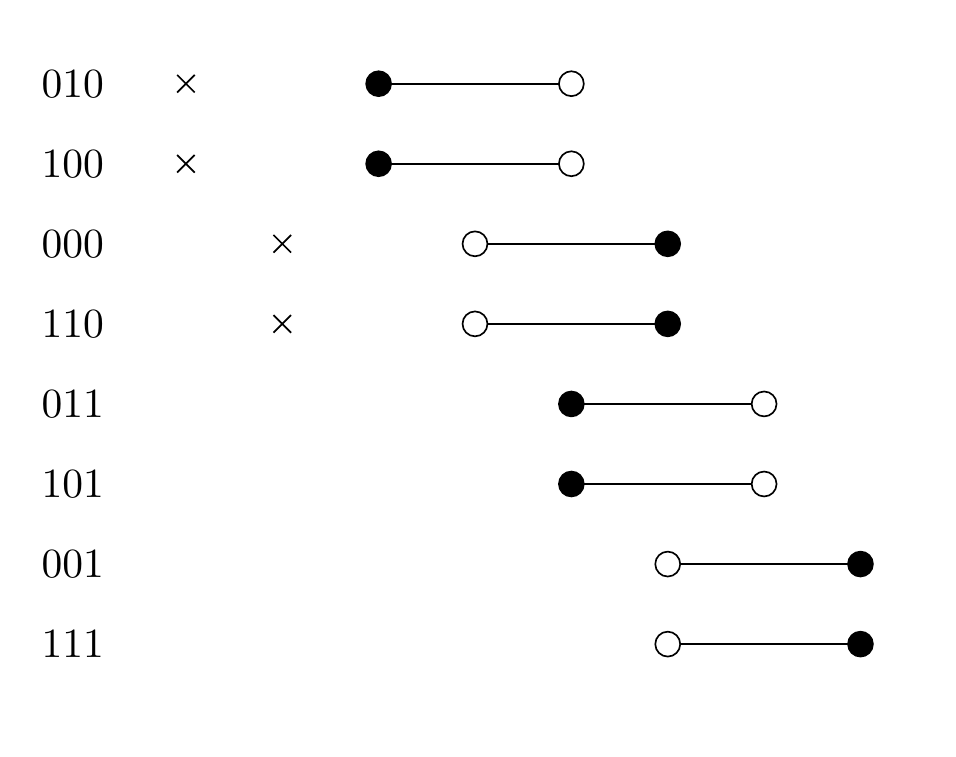
\begin{tikzpicture}[scale=1.5]
                \begin{axis}[
                        xticklabels={},
                        yticklabels={},
                        extra y ticks={1, 2, 3, 4, 5, 6, 7, 8},
                        extra y tick labels={$111$, $001$, $101$, $011$, $110$, $000$, $100$, $010$},
                        ytick style={draw=none},
                        xtick style={draw=none},
                        axis line style={draw=none}
                ]
                \addplot[
                    scatter,
                    scatter src=explicit symbolic,
                    mark size=3,
                    scatter/classes={
                        empty={mark=*, fill=white},
                        filled={mark=*, fill=black},
                        old={mark=x, fill=white}
                    },
                    nodes near coords*={\Label},
                    visualization depends on={value \thisrow{label} \as \Label}
                ]
                table [meta=class] {
                        x y class label
                        
                        1 8 old \empty
                        
                        3 8 filled
                        5 8 empty 
                        
                        1 7 old
                        
                        3 7 filled 
                        5 7 empty
                        
                        2 6 old 
                        
                        4 6 empty
                        6 6 filled
                        
                        2 5 old
                        
                        4 5 empty 
                        6 5 filled
                        
                        5 4 filled
                        7 4 empty
                        
                        5 3 filled 
                        7 3 empty
                        
                        6 2 empty
                        8 2 filled
                        
                        6 1 empty 
                        8 1 filled
                        };
                \end{axis}
            \end{tikzpicture}
            \caption{$\preceq_{p \ast \alpha \ast \beta}$ for $\beta = (p \vee q) \wedge (\neg p \vee \neg q)$}
            \label{fig:example-preceq-revised-alien2}
    \end{figure}
    
For the initial tpo $\leq$ there was no possible evidence that would change the plausibility ordering between worlds where the victim is an alien and worlds where they are not. That was reflected by the new tpo $\leq_{\alpha}^{\ast}$ that even with direct evidence for alien life did not change the judges plausibility orderings. But because of the revision of $\preceq$ to $\preceq_{p \ast \alpha}$ the evidence changed the acceptance of the judge to belief we are not alone in the universe. After receiving $\beta$ the judge even considers the $[r]$-worlds $\{011, 101\}$ more likely than the $[\neg r]$-worlds $\{000, 110\}$!

(Luckily due to the existence of $[\beta]$-worlds $\{010, 100\}$ the belief set of the judge still does not include $r$ and rationality prevails.)
\end{example}

% TODO write Discussion
\section{Discussion}
\label{section:discussion}
% TODO *6,*7 seem weird, no different "strength" of evidence? maybe revising multiple time by the same evidence should that be? otherwise revising multiple times by same evidence is also weird because it changes things and is not idempotent, discuss 5 with it being equal when sticks - and + are same rank?! 
\newpage

\typeout{}
\bibliographystyle{plain}
\bibliography{references}

\newpage

\section*{Erklärung}
Ich erkläre, dass ich die schriftliche Ausarbeitung zum Seminar selbstständig und ohne unzulässige Inanspruchnahme Dritter verfasst habe. Ich habe dabei nur die angegebenen Quellen und Hilfsmittel verwendet und die aus diesen wörtlich oder sinngemäß entnommenen Stellen als solche kenntlich gemacht. Die Versicherung selbstständiger Arbeit gilt auch für enthaltene Zeichnungen, Skizzen oder graphische Darstellungen. Die Ausarbeitung wurde bisher in gleicher oder Ähnlicher Form weder derselben noch einer anderen Prüfungsbehörde vorgelegt und auch nicht veröffentlicht. Mit der Abgabe der elektronischen Fassung der endgültigen Version der Ausarbeitung nehme ich zur Kenntnis, dass diese mit Hilfe eines Plagiatserkennungsdienstes auf enthaltene Plagiate geprüft werden kann und ausschließlich für Prüfungszwecke gespeichert wird.

\end{document}